\section{\gemini\ design \& implementation}
\label{ch:redblue:sect:gemini}

In this section we describe the design and implementation of
  \gemini, a prototype architecture that enables applications to run
  under \RBc.

\subsection{Design rationale}
As we saw in Section~\ref{ch:redblue:sect:casestudies},
some original operations may produce either \blue\ or \red\ \shadow\ \operations\
depending on the current system state and the user input they are observing. 
A nav{\" i}e solution would be to coordinate all generator operations that may produce
a \red\ shadow. This solution imposes more restrictions than
what \RBCN\ exactly needs, i.e., all relevant \shadow\ \operations\ even including
those blue ones would be serialized w.r.t each other. As a result, it
offsets the goal of \RBCN\ of only paying a performance penalty when strong consistency
is needed. To avoid this, we instead optimistically run 
the \initial\ \operation\ at its primary site in the first place,
and then speculatively generate a tentative shadow operation based on the local state and user input.
If the corresponding \shadow\ \operation\ is \blue, then a reply will be produced locally without
contacting remote replicas; Otherwise, replicas have to speak to
each other for establishing a total order among all \red\ shadow operations that are received,
and making sure that this \shadow\ \operation\ is generated
from a state reflecting all side effects introduced by all its preceding shadow operations. Therefore,
a \red\ tentative \shadow\ \operation\ might rollback, when the local state
is different from the global state due to conflicts, and we need to restart
the process of generating another shadow operation.

\begin{figure}[t!]
  \centering
    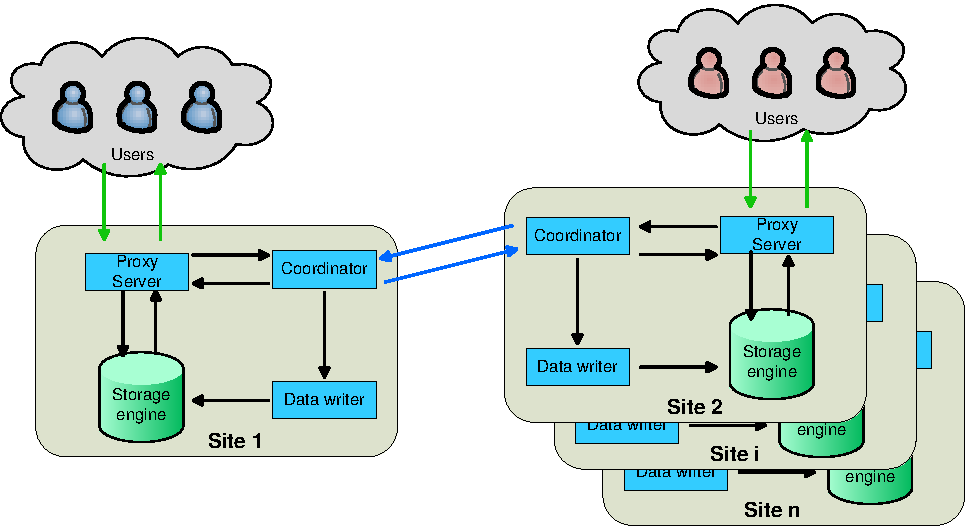
\includegraphics[width=0.95\columnwidth]{figures/redblue/GeminiArchi.pdf}
  \caption{Gemini system architecture. Blue arrows represent communication between sites,
black arrows indicate communication between system components within a site, and green
arrows correspond to communication between users and the replicated service.}
 \label{fig:geminiMultiDC}
\end{figure}

In addition, there are two requirements of executing generator operations: 1) they should
not interfere with other concurrent \transactions; and 2) there is no
need for them to make their identified side effects persistent. 
Given these observations, using a lock-based
concurrency control solution would be very conservative, since
granting locks to an \transaction\ may prevent other \transactions\ from making progress.
In summary, we resort to a form of optimistic concurrency control
(OCC)~\cite{Bernstein1987CCR} in \gemini, as we describe next. 
It is worth mentioning that the \gemini\ OCC slightly
deviates from the traditional textbook algorithm, since
our algorithm recognizes the fact that concurrent
\blue\ \shadow\ \operations\ are never conflicting with
all other \shadow\ \operations.

\if 0
In addition, under the \RBc\ model, \blue\ \transactions\ can never
conflict since they are assumed to concurrent red \transactions\ are
never conflicting with each other since they commute. In addition,
\initial\ \transactions\ should not interfere with other concurrent
\transactions.  Given these observations, using a lock-based
concurrency control solution would be very conservative, since
granting locks to a \transaction\ prevents other \transactions\ from
processing. As a result, we resort to optimistic concurrency control
(OCC)~\cite{Bernstein1987CCR} in \gemini, as we describe next.

\changebars{}
{
%\paragraph
{Extending commutativity}
% Identifying invariants requires us to analyze applications' sourcecode. The focus of this process is to check two essential parts of sourcecode normally used to express application invariants: \emph{if} statements embraced by synchronized primitives, and restrictions defined over data schemas (e.g., AUTOINCREMENT, UNIQUE attributes in MySQL). By doing so, we quickly identified two common invariants: a) id assigned must be unique; and b) the value of some state should not be negative.
We also observed that some \transactions\ were not immediately commutative due to implementation issues rather than to intrinsic non-commu-tativity issues.
One example is the implementation of uni-que identifiers---in the base centralized application we have used, unique identifiers are assigned using a monotonic counter stored in the database.
%When using this approach in our system, if the identifier is generated in the initial \transaction, concurrent initial \transactions\ running in %different sites could generate the same identifier. If the identifier is generated in the \shadow\ \transaction, \shadow\ \transactions would have %to execute in the same order in all replicas - i.e., they should be labeled blue.
We addressed this issue by associating each unique identifier with a site-specific prefix so that it is globally unique.
A second example is the case where commutativity is impeded by non-determinism in the operations executed in a transaction. This negative %impact can be easily solved by solving the non-determinism in the initial transaction and encoding the expected result into \shadow\ \operation.
impact can be easily solved by encoding the results produced by these operations into the corresponding \shadow\ \operations.
}
\fi

%As shown in Figure~\ref{fig:geminiMultiDC}, a single-site
%\nuno{************* new try starts here *************************************************************}

\subsection{System overview}
We implemented the \gemini\ storage system to provide \RBc. As shown in Figure~\ref{fig:geminiMultiDC}, each \gemini\ site consists of four components:
a storage engine, a proxy server, a concurrency coordinator, and a
 data writer. A multi-site deployment is constructed by replicating
 the single data center components across multiple sites.

The basic flow of user requests through the system is straightforward.
A user issues requests to a {\em proxy server} located at the closest
site. The proxy server processes a request by executing the \initial\ \operation\ of an
appropriate application transaction, which is implemented as a single
\gemini\ original \operation, comprising multiple data accesses; individual
data accesses within a \initial\ \operation\ execute in a temporary
private scratchpad, providing a virtual private copy of
  the service state. The original data lies in a {\em storage engine}, which provides a standard
storage interface. In our implementation, the storage
  engine is a relational database, and scratchpad operations are
  executed against a set of non-shared in-memory tables. Upon completion of the
\initial\ \operation, the proxy server sends the produced
\shadow\ \operation\ on to the {\em concurrency coordinator} to admit
or reject this \operation\ according to \RBc. The concurrency
coordinator notifies the proxy server if the \shadow\ \operation\ is accepted
or rejected.  Additionally, accepted \shadow\ \operations\ are
appended to the end of the local legal causal serialization and propagated to remote
sites and to the local {\em data writer} for execution against the
storage engine.  When a \shadow\ \operation\ is rejected, the proxy
server re-executes the \initial\ \operation\ and restarts the process.

%\subsection{Technical details (alternative take)}
%\subsection{Optimistic concurrency control}\cheng{better to be 'Technical details', as the following
%text covers ideas including OCC but beyond it.}

\subsection{Ordering and replicating transactions}

%Gemini relies on optimistic concurrency control
%(OCC)~\cite{Bernstein1987CCR} to run
%\initial\ \transactions\ to generate the corresponding \shadow\ \operations\ and
%to make a decision on whether coordination is required without blocking on
%either concurrent local or remote \operations.  
%\changebars{} {The
%  \initial\ \transaction\ runs in a private scratchpad that implements
%  a virtual copy of the storage engine. }

The most sophisticated part of \gemini\ is how to establish a
\RBo\ of shadow operations generated by different replicas
and to replicate all these shadow operations in site-dependent
causal legal serializations at every replica. First, \Gemini\ uses timestamps to determine if 
\operations\ can complete successfully, i.e., operations can be
admitted to appear in the corresponding global \RBo. Timestamps are logical clocks~\cite{Lamport1978Time} of
the form $\langle \langle b_0, b_1, \ldots, b_{k-1}\rangle, r\rangle$,
where $b_i$ is the local count of \shadow\ \operations\ initially
executed by site $i$ and $r$ is the global count of
\red\ \shadow\ \operations.  To ensure that different sites do not
choose the same \red\ sequence number (i.e., all
  \red\ \operations\ are totally-ordered) we use a simple token
passing scheme: only the coordinator in possession of a unique
\red\ token is allowed to increase the counter $r$ and approve
\red\ \operations.  In the current prototype, a coordinator holds
onto the \red\ token for up to 1 second
before passing it along.

When a \initial\ \transaction\ completes, the corresponding
\shadow\ \operation\ is produced and colored according
to the templates and classification results presented in Section~\ref{ch:redblue:sect:casestudies}.
Then, the colored \shadow\ \operation\ is passed to the coordinator for
determining if this \operation\ can be accepted to the global redblue order. 
If it is \blue, the coordinator only performs a read coherence check, i.e.,
the logical timestamps of the data items in its read set
are less than or equal to the begin timestamp assigned when the corresponding transaction started.
\changebars{If the pending shadow operation is \red, then the coordinator has to verify if the state where 
the operation was generated from reflects the effects of the set of accepted 
\red\ \shadow\ \operations\ that precede it according to some total order established by
the token assignment scheme. To do this, the coordinator has to wait
until the red token has reached its site, i.e., \red\ \shadow\ \operations\ initially executed
at the previous red token holder site have been applied locally. Then, the coordinator
performs a read-write conflict check consisting of two steps: a) acquiring locks for data items in the pending
shadow operation's write set, in order to prevent local concurrent pending red shadow operations
from proceeding; and b) checking if the data items in the pending shadow operation's read set are not locked
and have not been modified by any other accepted shadow operations between the time when
the transaction generating the pending shadow operation started and the check was triggered.}{}

Upon successful completion of the above checks, the coordinator assigns the 
corresponding \shadow\ \operation\ a timestamp that is com\-po\-nent-wise equal
to the latest \operation\ that was incorporated at its site, and
increments its \blue\ and, if this \shadow\ \operations\ is
  \red, the \red\ component of the logical
timestamp. This timestamp determines the position of the
\shadow\ \operation\ in the \RBo, with the normal rules
that determine that two operations are partially ordered if one is
equal to or dominates the other in all components. It also allows
sites to know when it is safe to incorporate remote shadow
transactions: they must wait until all \shadow\ \transactions\ with
smaller timestamps have already been incorporated in the local state
of the site. When a remote \shadow\ \operation\ is applied at a site, the most recent local logical clock maintained
by this site will be replaced with the entry-wise max of its current value
and the timestamp shipped with that \shadow\ \operation. This captures dependencies that span local and remote \transactions. 

%it is assigned a new timestamp that is the
%entry-wise max of the timestamp assigned to the
%\shadow\ \transaction\ in the initial site and the local timestamps of
%accessed data objects. This captures dependencies that span local and remote \transactions.

\paragraph{Read-only \shadow\ \operations.} 
 As a performance optimization, \blue\ \shadow\ \operations\ can be
 marked as read-only. Read-only \shadow\ \operations\ receive special
 treatment from the coordinator: once the \initial\ \operation\ passes
 the coherence and causality checks, the proxy is notified that the
 \shadow\ \operation\ has been accepted but the
 \shadow\ \operation\ is {\em not} incorporated into the local
 serialization or global \RBo. Thus, read-only \operations\ are
never sent across sites.

\if 0
\paragraph{Scratchpad.} \changebars{Another interesting aspect of our
architecture is to implement isolated scratchpads inside MySQL for making
the execution of generator and shadow generations not interfere with
each others. As MySQL implements a lock-based concurrency control algorithm
rather than OCC, we were experiencing deadlocks and long waiting
in the initial design. To achieve the goal of optimizing
user-observed latency, we changed the lock-based implementation
into a form of OCC by creating a
set of scratchpads (sandboxes). Each scratchpad consists of 
a few in-memory temporary tables, which is one-to-one mapping
to real tables in the database. All changes determined by executing \initial\ \operations\ are
first stored in the corresponding temporary tables. All subsequent reads inside
the same \initial\ \operation\ will return the result obtained by merging
 the data from in-memory tables and the real tables. This is how we prevent
from locking actual items in real tables prior to commits.
When a pair of \initial\ and \shadow\ \operations\ succeeds, changes will be
introduced to real tables and the data in temporary tables will be simply discarded. Since temporary tables
are always remaining in memory and not shared across scratchpads, reads from and writes to them can be fast.}{}
\fi

%% %new
%% \changebars{}
%% %old
%% {
%% \subsection{Implementation}
%% The \gemini\ system consists of 10k lines of Java code and utilizes
%% the Netty asynchronous i/o library\cite{Netty}.  We
%% \changebars{use}{augment the main
%% system with} a modified JDBC driver to facilitate the integration of
%% \gemini\ into the MySQL based applications (with
%% \transaction\ boundaries that already defined) discussed in
%% \S\ref{sect:casestudies}.
%% }
%% %done

%\subsection{Unique number generation}
%\cheng{adding unique id generator}

\subsection{Failure handling}
\label{sect:handleFaults}
The current \gemini\ prototype is designed to demonstrate the
performance potential of \RBc\ in geo-replicated environments and as
such is not implemented to tolerate faults of either a local (i.e.,
within a site) or catastrophic (i.e., of an entire site) nature.
Addressing these concerns is orthogonal to the primary contributions
of this work, nonetheless we briefly sketch mechanisms that could be
employed to handle faults.
%% {a variety of obvious
%% failure modes.  We note that we do not propose any new fault
%% tolerant mechanisms and instead identify where standard techniques
%% could be used to buttress the reliability of our architecture.}

\paragraph{Isolated component failure.}  The \gemini\ architecture consists 
of four main components at each site, each representing a single point
of failure.  Standard state machine replication
techniques~\cite{Lamport1978Time,Schneider1990RSM} can be employed to
make each component robust to failures.
%\changebars{}{The replication of stateless
%components (namely the proxy and the data writer) can be further
%simplified by obviating the serialization provided by state machine replication.}

\paragraph{Site failure.} Our \gemini\ prototype relies on a simple 
ring-exchange for serializing all \red\ shadow operations. Thus the failure of a single
site is enough to stop the token exchange and prevent future
\red\ transactions from completing. To avoid halting the system upon a site failure,
a fault tolerant consensus protocol like Paxos~\cite{Lamport1998Paxos}
can regulate \red\ tokens.

\paragraph{\Operation\ propagation.}  \Gemini\ relies on each site to
 propagate its own local \transactions\ to all remote sites.  A
 pair-wise network outage or failure of a site following the
 replication of a \transaction\ to some but not all of the sites
could prevent sites from exchanging
 \transactions\ that depend on the partially replicated \transaction.
 This can be addressed using standard techniques for exchanging
 causal logs~\cite{Mahajan2010Depot, Ahamad1994causalmemory,
   Terry1995Managing, Petersen1997Flexible} or reliable multicast~\cite{Floyd1997Multicast}.

\paragraph{Cross-session monotonicity.} The proxy that each user connects to enforces the
  monotonicity of user requests within a
  session~\cite{Terry1994Session}. However, a
failure of that proxy, or the user connecting to a different site may result in a
subset of that user's operations not carrying over. This can be addressed by allowing the user to
specify a ``last-read'' version when starting a new session or
requiring the user to cache all relevant
requests~\cite{Mahajan2010Depot} in order to replay them when connecting
to a new site.

\subsection{Implementation}
The \gemini\ system consists of 10k lines of Java code~\footnote{The lines of code is
measured by {\tt cloc}~\cite{codecounter}.}, and uses
MySQL~\cite{MySQL} as its storage backend, and 
the Netty asynchronous i/o library\cite{Netty} for communication.  We
extended a JDBC driver~\cite{JdbcDriver} so that it is able to facilitate the integration of
\gemini\ into the MySQL based applications discussed in
Section~\ref{ch:redblue:sect:casestudies}. The sourcecode is available at~\cite{GeminiSource}.


 
